\documentclass[11pt,english]{article}

%%%%%%%%%%%%%%%%%%%%%%%%%%%%%%%%%%%%%%%%%%%%%%%%%%%%%%%%%%%
% Packages
%%%%%%%%%%%%%%%%%%%%%%%%%%%%%%%%%%%%%%%%%%%%%%%%%%%%%%%%%%%

% Package imports are stored in /assets/base-packages.tex
% Packages specific to this pset can be imported here.

\listfiles
% paper size & margins
\usepackage{fullpage}
\usepackage[showframe=false,margin=1in]{geometry}
\parindent=0pt

% font management
\usepackage{relsize}
\usepackage[T1]{fontenc} % for properly hyphenating words with accented chars
\usepackage[latin1]{inputenc}
\usepackage{babel}

% figure management
\usepackage{epsfig}
\usepackage{graphicx}
\usepackage{wrapfig}
\usepackage{subfig}
%\usepackage{subfigure}
\usepackage[belowskip=0pt,aboveskip=0pt,font=small]{caption}
%\usepackage{subcaption}
\setlength{\intextsep}{7pt plus 0pt minus 0pt}

% math
\usepackage{amsmath, amsthm, amssymb}
%\usepackage{amstext}
\usepackage{textcomp}
\usepackage{stmaryrd}
\usepackage{upgreek}
\usepackage{bm}
\usepackage{cases}
\usepackage{mathtools}

% assorted
\usepackage{url}
\usepackage{breakurl}
\usepackage[colorlinks=true]{hyperref}
\usepackage{xspace}
\usepackage{comment}
\usepackage{color}
\usepackage{afterpage}
\usepackage[normalem]{ulem}
\usepackage{enumitem}



%%%%%%%%%%%%%%%%%%%%%%%%%%%%%%%%%%%%%%%%%%%%%%%%%%%%%%%%%%%
% Shortcuts

%%%%%%%%%%%%%%%%%%%%%%%%%%%%%%%%%%%%%%%%%%%%%%%%%%%%%%%%%%%
\usepackage{mysymbols}
%%% load AMS-Latex Package
\usepackage{amsmath,amsfonts}
\usepackage{amsthm,amssymb,amsopn}
\usepackage{bm} % bold symbol
\usepackage{bbm}

% define fonts
\newcommand{\vct}[1]{\boldsymbol{#1}} % vector
\newcommand{\mat}[1]{\boldsymbol{#1}} % matrix

%%%% Special math symbols
\newcommand{\field}[1]{\mathbb{#1}}
\newcommand{\R}{\field{R}} % real domain
\newcommand{\C}{\field{C}} % complex domain
\newcommand{\F}{\field{F}} % functional domain
%\newcommand{\T}{^{\top}\!\!} % transpose
\newcommand{\T}{^{\textrm T}} % transpose
\newcommand{\TN}{^{-\textrm T}} % transpose
\newcommand{\Lagr}{\mathcal{L}}


%%% define constant
\newcommand{\cst}[1]{\mathsf{#1}}

%% operator in linear algebra, functional analysis
\newcommand{\inner}[2]{#1\cdot #2}
%\newcommand{\norm}[1]{\|#1\|}
\newcommand{\twonorm}[1]{\|#1\|_2^2}
% operator in functios, maps such as M: domain1 --> domain 2
\newcommand{\Map}[1]{\mathcal{#1}}

% operator in probability: expectation, covariance,
\newcommand{\ProbOpr}[1]{\mathbb{#1}}
% independence
\newcommand\independent{\protect\mathpalette{\protect\independenT}{\perp}}
\def\independenT#1#2{\mathrel{\rlap{$#1#2$}\mkern2mu{#1#2}}}
% conditional independence
\newcommand{\cind}[3]{{#1} \independent{#2}\,|\,#3}
% conditional expectation
\newcommand{\cndexp}[2]{\ProbOpr{E}\,[ #1\,|\,#2\,]}

% operator in optimization
%\DeclareMathOperator{\argmax}{arg\,max}
%\DeclareMathOperator{\argmin}{arg\,min}
%\newcommand{\todo}[1]{{\color{red}#1}}


% environment
\newtheorem{thm}{Theorem}

\newcommand{\eat}[1]{}

\newcommand{\hide}[1]{}
%\newcommand{\solution}{{\Large \vspace{5mm} \textbf{{\color{red}Solution:}}\newline\newline}}

\newcommand{\diff}{\mathop{}\!\mathrm{d}}
\newcommand{\Vop}{\textrm{T}}
\newcommand{\norminf}[1]{\norm{#1}_\infty}

% definitions for PS4
\newcommand{\vecy}{\ensuremath{\mathbf{y}}\xspace}
\newcommand{\vecx}{\ensuremath{\mathbf{x}}\xspace}
\renewcommand{\argmax}{\operatornamewithlimits{argmax}}
\newcommand{\startsym}{\mbox{\scriptsize \texttt{<s>}}\xspace}
\newcommand{\stopsym}{\mbox{\scriptsize \texttt{</s>}}\xspace}
\newcommand{\best}{\ensuremath{\mathit{best}}\xspace}
\newcommand{\bestuptoi}{\ensuremath{\texttt{best}_{\leq i}}\xspace}
\newcommand{\bestuptot}{\ensuremath{\texttt{best}_{\leq t}}\xspace}
\newcommand{\completed}{\ensuremath{\texttt{comp}}\xspace}
\newcommand{\toptop}{\operatornamewithlimits{\mathbf{top}}}
\newcommand{\tuple}[1]{\ensuremath{\langle {#1} \rangle}}
\newcommand{\xuptot}{\ensuremath{\mathit{x}_{\leq t}}\xspace}


\renewcommand{\hide}[1]{}
\usepackage{graphicx}
%%%%%%%%%%%%%%%%%%%%%%%%%%%%%%%%%%%%%%%%%%%%%%%%%%%%%%%%%%%
% Title / Author
%%%%%%%%%%%%%%%%%%%%%%%%%%%%%%%%%%%%%%%%%%%%%%%%%%%%%%%%%%%
\begin{document}
\title{CS 4644/7643: Deep Learning\\
Spring 2025 \\
Problem Set 1}

% NOTE: Any changes to instructor, TAs, or piazza link should be done in the file below
\author{Instructor: Zsolt Kira \\
TAs: Wei Zhou, Aryan Sarswat, Woo Chul Shin, Elias Cho, \\Haotian Xue, Sri Siddarth Chakaravarthy Prakash, Neelabh Sinha, David He, \\ Sriharsha Kocherla, Pratham Mehta, Ayush Patel, Cari He\\
Discussions: \url{https://piazza.com/class/m5k29i4gzsf4ab/}}
\date{Deadline: 11:59pm January 31st, 2025}
\maketitle

\paragraph*{Instructions}
\begin{enumerate}
\item We will be using Gradescope to collect your assignments.  Please read the following instructions for submitting to Gradescope carefully!
     \begin{itemize}
          % \item
               % This assignment has 10 total problems/sub-problems. Questions 1-7 are theory questions, while 8-10 are programming
               % questions. 
          \item
               For the \textbf{HW1 Theory} component on Gradescope, upload one single PDF containing the answers to all the theory questions. \textbf{However, the solution to each problem/subproblem must be on a separate page. When submitting to Gradescope, please make sure to mark the page(s) corresponding to each problem/sub-problem.}
          \item
               For the \textbf{HW1 Coding} component on Gradescope, please use the \texttt{collect\_submission.ipynb} notebook provided and upload the resulting \textbf{hw1\_code\_submission.zip} on Gradescope. Please make sure you have saved the most recent version of your code.
          \item
               For the \textbf{HW1 Writeup} component on Gradescope, please use the \texttt{collect\_submission.ipynb} script provided and upload the resulting \textbf{hw1\_notebook\_submission.pdf} on Gradescope.
          \item
               Note: This is a large class and Gradescope's assignment segmentation features are essential.
               Failure to follow these instructions may result in parts of your assignment not being graded.
               We will not entertain regrading requests for failure to follow instructions.

               % Please read \url{https://stats200.stanford.edu/gradescope_tips.pdf} for additional information on submitting to Gradescope.
     \end{itemize}

\item
     \LaTeX'd solutions are strongly encouraged (solution template
     available in the zip file in HW1-Theory under the Assignments tab on Canvas), but scanned handwritten copies are acceptable. Hard copies are \textbf{not} accepted.


\item We generally encourage you to collaborate with other students.

You may talk to a friend,
discuss the questions and potential directions for solving them. However, you need to write
your own solutions and code separately, and \emph{not} as a group activity.
Please list the students you collaborated with. \\ \\

\end{enumerate}
\newpage

%%%%%%%%%%%%%%%%%%%%%%%%%%%%%%%%%%%%%%%%%%%%%%%%%%%%%%%%%%%
% Body
%%%%%%%%%%%%%%%%%%%%%%%%%%%%%%%%%%%%%%%%%%%%%%%%%%%%%%%%%%%

\section{Collaborators [0.5 points]}

Please list your collaborators and assign this list to the corresponding section of the outline on Gradescope. If you don't have any collaborators, please write 'None' and assign it to the corresponding section of the Gradescope submission regardless.


\section{Optimization}

\begin{enumerate}[start]

\item
\textbf{[2 points]}
Let $f(\mathbf{x})$ be a function, where $\mathbf{x} \in \mathbb{R}^d$.
The \textit{level surface} of a function is the set of points with the same value of function, \ie
\begin{equation}
    L_c = \left\{ \mathbf{x} \mid f(\mathbf{x}) = c \right\} \label{q11.ls}
\end{equation}
for some c $\in$ $\mathbb{R}$. 

\begin{figure}[h!]
    \centering
    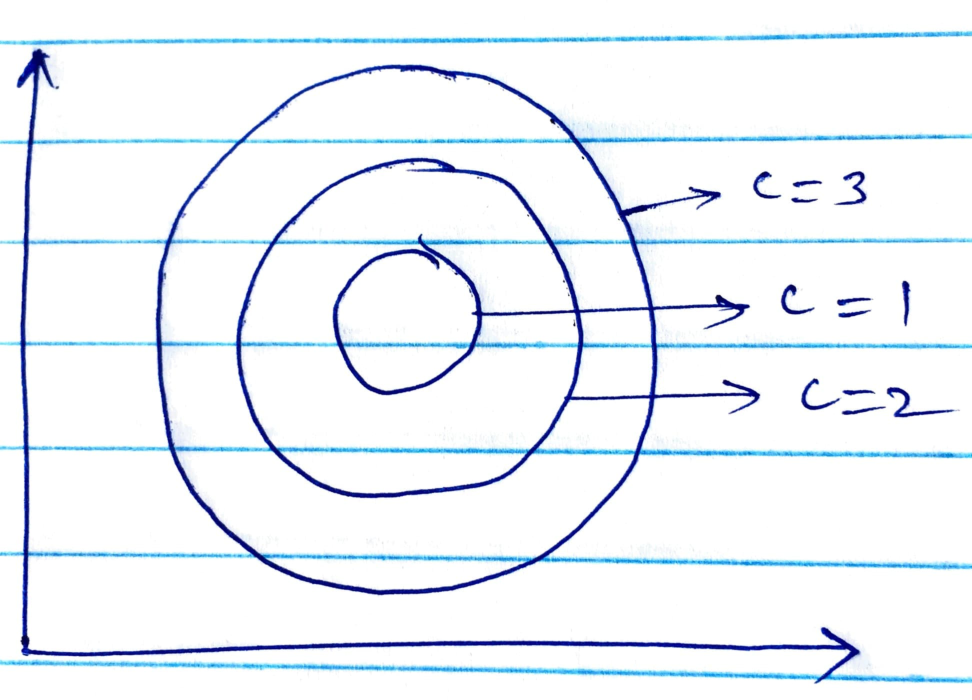
\includegraphics[scale=0.5]{circle_dl.pdf}
\end{figure}

The above figure shows level surfaces for different values of c for a 2-dimensional case. The points on the perimeter of each curve illustrate the set of points sharing the same value, i.e. $f(x_1, x_2) = c$.

Recall that a gradient vector is defined as $\nabla f = \left[ \frac{\partial f}{\partial x_1}, \frac{\partial f}{\partial x_2}, ..., \frac{\partial f}{\partial x_d} \right]$.

Consider a specific point $\mathbf{x}_0 \in \mathbb{R}^d$. Let us denote the level surface passing through this point by $L_{f(\mathbf{x_0})}$. Let us denote the gradient vector at $\mathbf{x_0}$ by $\nabla f_0$. 

Now, consider an arbitrary curve $\mathbf{r}(t) = \left[x_1(t); x_2(t); \ldots, x_d(t)\right]$ (parameterized by a scalar $t$) that passes through $\mathbf{x}_0$, 
\ie $\mathbf{r}(t_0) = \mathbf{x_0}$ for some $t_0 \in \mathbb{R}$. Furthermore, 
the curve $\mathbf{r}(t)$ lies within the level surface passing through $\mathbf{x}_0$, \ie $\mathbf{r}(t) \in L_{f(\mathbf{x_0})}, \,\, \forall t$.  

Recall that the \emph{tangent} to a curve is defined as $\frac{\del \mathbf{r}}{\del t}$. 

%lies within the level surface, \ie $\mathbf{r}(t) \in L$  where $\mathbf{r}(0) = \mathbf{x_0}$, i.e. it passes through $x_0$. 

With all that context and notation behind us, now comes the `fun' part -- 
show that $\nabla f_0$ is orthogonal to the tangent of $\mathbf{r}(t)$ at $t_0$. 

Now, please describe in non-technical language what you have just proven. Why might we care about this in the context of deep learning? 



\item
\textbf{[2 points]}

Consider a (not necessarily convex) differentiable function $g : \mathbb{R}^{n} \rightarrow \mathbb{R}$. $g$ has a local minimum at some $\mathbf{w}^{t}$ if there exists some $\gamma > 0$ such that for all $\mathbf{w} \in \mathbb{R}^{n}$, $\norm{\mathbf{w}^{t} - \mathbf{w}}_{2} < \gamma \Rightarrow g(\mathbf{w}^{t}) \leq g(\mathbf{w})$.

Prove that if $g$ has a local minimum at some $\mathbf{w}^{t}$ then the gradient at $\mathbf{w}^{t} = 0$, and that the converse
is not necessarily true.

\item
\textbf{[3 points]}

Prove that if a differentiable function $g : \mathbb{R}^{n} \rightarrow \mathbb{R}$ is convex and the gradient
at some $\mathbf{w}^*$ is 0, then $\mathbf{w}^*$ is the global minimum of $g$ (\textbf{Grading note: Students should NOT be allowed to use first order condition without proof}).

\item
\textbf{[2 points]}

During lecture 3, we discussed the softmax function $\mathbf{s}(\mathbf{z})$, which takes a vector input $\mathbf{z}$ and outputs a vector whose $i$th entry $s_i$ is

\begin{equation}
s_i = \frac{e^{z_{i}}}{\sum_{k} e^{z_{k}}}
\end{equation}

The input vector $\mathbf{z}$ to $\mathbf{s}(\cdot)$ is sometimes called the ``logits'', which just means the unscaled output of previous layers. Derive the gradient of $\mathbf{s}$ with respect to the logits, \ie derive $\frac{\partial \mathbf{s}}{\partial \mathbf{z}}$. 
Consider re-using your work from HW0.

\item
\textbf{[3 points: Extra credit for both 4644 and 7643]}

Recall that a ($d-1$)-dimensional simplex is defined as: 
\begin{equation}
    \Delta_{d - 1} = \{\mathbf{p} \in \mathbb{R}^{d} \mid \mathbf{1}^{T}\mathbf{p} = 1 \text{ and } p_i \ge 0 \,\, \forall i \in \{1,\ldots,d\} \}
\end{equation}

In this question, you will develop an interpretation of softmax as a projection operator -- that it projects an arbitrary point $\mathbf{x} \in \mathbb{R}^d$ onto the interior of the $d - 1$ simplex. Specifically, let $\mathbf{s}(\mathbf{x})$ denote the softmax function (as defined above). Now prove that, 


\begin{align}
    \mathbf{s}(\mathbf{x}) =  \argmin_{\mathbf{y} \in \mathbb{R}^d} &\quad  -\mathbf{x}^{T}\mathbf{y} - H(\mathbf{y}) \\ 
     \st & \quad \mathbf{1}^{T}\mathbf{y} = 1, \quad 0 \le y_i \le 1 \quad \forall i
\end{align}

where $H$ is the entropy function: 

\begin{equation}
    H(\mathbf{y}) = - \sum_{i}y_{i}\log(y_{i})
\end{equation}

Now, what does this formal interpretation tell you about the softmax layer in a neural network? 
Hint: Look at the KKT conditions.


\end{enumerate}

\section{Directed Acyclic Graphs (DAG)}


One important property for a feed-forward network, as discussed in the lectures, is that it must be a directed acyclic graph (DAG). Recall that a \emph{DAG is a directed graph that contains no directed cycles}. We will study some of its properties in this question.

Let's define a graph $G=(V, E)$ in which $V$ is the set of all nodes as $\{v_1, v_2, ..., v_i, ... v_n\}$ and $E$ is the set of 
edges $E = \big\{e_{i,j} = (v_i, v_j) \mid v_i, v_j \in V \big\}$.

A \emph{topological order of a directed graph} $G=(V, E)$ is an ordering of its nodes as $\{v_1, v_2, ..., v_i, ... v_n\}$ so that for every edge $(v_i, v_j)$ we have $i < j$.


There are several lemmas that can be inferred from the definition of a DAG. One lemma is: if $G$ is a DAG, then $G$ has a node with no incoming edges.   


\begin{enumerate}[resume]

\item
\textbf{[3 points]}

Prove that if the graph $G$ is a DAG, then $G$ has a topological ordering.

\item
\textbf{[3 points]}

Prove that if the graph $G$ has a topological order, then $G$ is a DAG.

\end{enumerate}

\section{Paper Review}

%%%% Point values defined in the file below %%%%

The first of our paper reviews for this class comes from a NeurIPS 2019 paper on the topic \textbf{`Weight Agnostic Neural Networks'} by \textbf{Adam Gaier} and \textbf{David Ha} from Google Brain.

The paper presents an interesting proposition that, through a series of experiments, re-examines some fundamental notions about neural networks - in particular, the comparative importance of architectures and weights in a network's predictive performance. 

The paper can be viewed \href{https://arxiv.org/abs/1906.04358}{here}.
There's also a helpful \href{https://weightagnostic.github.io/}{interactive webpage} with intuitive visualizations to help you understand its key concepts better. 

The evaluation rubric for this section is as follows:

\begin{enumerate}[resume]
\item
\textbf{[2 points]}
Briefly summarize the key contributions, strengths and weaknesses of this paper.

\item
\textbf{[2 points]}
What is your personal takeaway from this paper? This could be expressed either in terms of relating the approaches adopted in this paper to your traditional understanding of learning parameterized models, or potential future directions of research in the area which the authors haven't addressed, or anything else that struck you as being noteworthy. 
\end{enumerate}

\textbf{Guidelines}: Please restrict your reviews to no more than 350 words (total length for answers to both the above questions).

\section{Implement and train a network on MNIST}

\begin{enumerate}[resume]

\item
\textbf{[22 points]}

Please refer to the instructions in the starter code zip file available on Canvas, in HW1-Coding under the Assignments tab, to get started. Please remember to label your pages after you submit your writeup.

% You will need to combine your solutions to the previous questions with the report of your coding section and submit them together on Gradescope. You can use an online pdf combiner such as \href{https://combinepdf.com/}{this one}. 




\end{enumerate}

\end{document}